\documentclass[a4paper,12pt]{article}
\usepackage{graphicx}
\usepackage{enumerate}
\usepackage{geometry}
\usepackage{times}
\geometry{legalpaper, portrait, margin=.75in}

\begin{document}

\begin{flushright}

\vspace{1.1cm}

{\bf\Huge Lab 4}

\rule{0.25\linewidth}{0.5pt}

\vspace{0.5cm}
%Put Authors
Justin Ely
\linebreak
\newline
%Put Author's affiliations
\footnotesize{615.202.81.FA15 Data Structures \\}
\vspace{0.5cm}
% Date here below
06 December, 2015
\end{flushright}

\noindent\rule{\linewidth}{1.0pt}

%%%%%%%%%%%%%%%%%%%%%%%%%%%%%%%%%%%%%%%%%%%%%%%%%%%%%%%%%%

\section{Comments}
Sorting algorithms are a key component to computer science, not simply because sorting is a commonly-performed task, but because of the knowledge gained through examining the various algorithms.  The development and usage of the different methods demonstrates clearly how limiting any particular application can be, and the lengths that need to be employed to be truly useful in all scenarios.

In this lab we mainly explored two sorting algorithms, quick sort and heap sort, with additional analysis on insertion sort and various implementations of quick sort.  From this exploration, we can see that the main factor in choosing a sorting algorithm is the number of elements to be sorted.  For small sorts any of the available methods will complete in fractions of a second, and would be a fine choice in anything but very optimized computations and repeated operations.  For larger file sizes however, the choice of algorithm can quickly change a solvable program into an insolvable one as the difference in execution times can vary by several orders of magnitude.


%%%%%%%%%%%%%%%%%%%%%%%%%%%%%%%%%%%%%%%%%%%%%%%%%%%%%%%%%%

\section{Design}
\subsection{Recursion vs Iteration}
I chose to do both the Heapsort and Quicksort as recursive algorithms.  A main driver for this was that a recursive quick sort was a requirement for other parts of the lab.  By starting off with a recursive function, some work could be saved.  Additionally, since quicksort and heapsort both can be easily understood in a recursive form, the development wasn't difficult.


\subsection{Enhancements}
My first enhancement was driven by the recursive implementation of the quicksort.  The default stack size for the JVM was insufficient  to sort some of the larger input arrays, so an optional runtime flag was added to the Makefile to increase the size.  By running the Driver for quick sort with '-Xss90m', files of more than 10,000,000 items can be sorted.  

To get a better grasp of the time-complexity, and to see when these algorithms can truly become prohibitive, files with up to 1,000,000 items were included in the analysis.  Additionally, input files that contained large numbers of repeated values were analyzed.

In addition to the recursive heap sort, a iterative version was completed as well.  Also timed insertion sort for analysis.

Unittests were added and used throughout development.  This was crucial to ensuring that any modifications to the sorting algorithms didn't cause a disruption in their ability to correctly sort data.  Additionally, the javadoc tool was used to provide documentation to the project.  However, due to the use of non-standard libraries for these functions, the ability to disable them was added to the given makefile.


\subsection{Limitations}
The main limitation is the restriction to integer type.  Both the main driver and the individual sorting methods are all limited to work with integer values.  The main program will only read integers from the input files, and the sorting algorithms are hard-coded to build and work with integer arrays and comparisons.  

As discussed in the Efficiency section, the current algorithms employed are a major limiting factor in the actual usefulness of the code.  Attempting to sort more than 1,000,000 items began to take multiple minutes to run, which limits the usefulness of the code.  However, in a real-world scenario, it's unclear how often datasets of such size are sorted.  

Though not a limitation of the algorithms, I find that the java language is very limiting in both command-line option parsing and function calling.  In particular, the ability to pass keyword arguments to both programs and functions would allow the code to be much more elegant.

%%%%%%%%%%%%%%%%%%%%%%%%%%%%%%%%%%%%%%%%%%%%%%%%%%%%%%%%%%

\section{Efficiency}


As discussed in the Enhancements section, both an iterative and recursive version of the heap sort was was implemented.  The analysis of the timing data for these two versions displays an interesting trend.  Though both versions show almost identical performance, for smaller datasets the iterative version is consistently faster than the recursive call.  This switches around for larger datasets, where the recursive call becomes consistently faster than the iterative version.  This indicates that the recursive method is actually quicker, but there is a small constant overhead that is only overcome with the larger file sizes.


\begin{figure}[h]
    \centering
    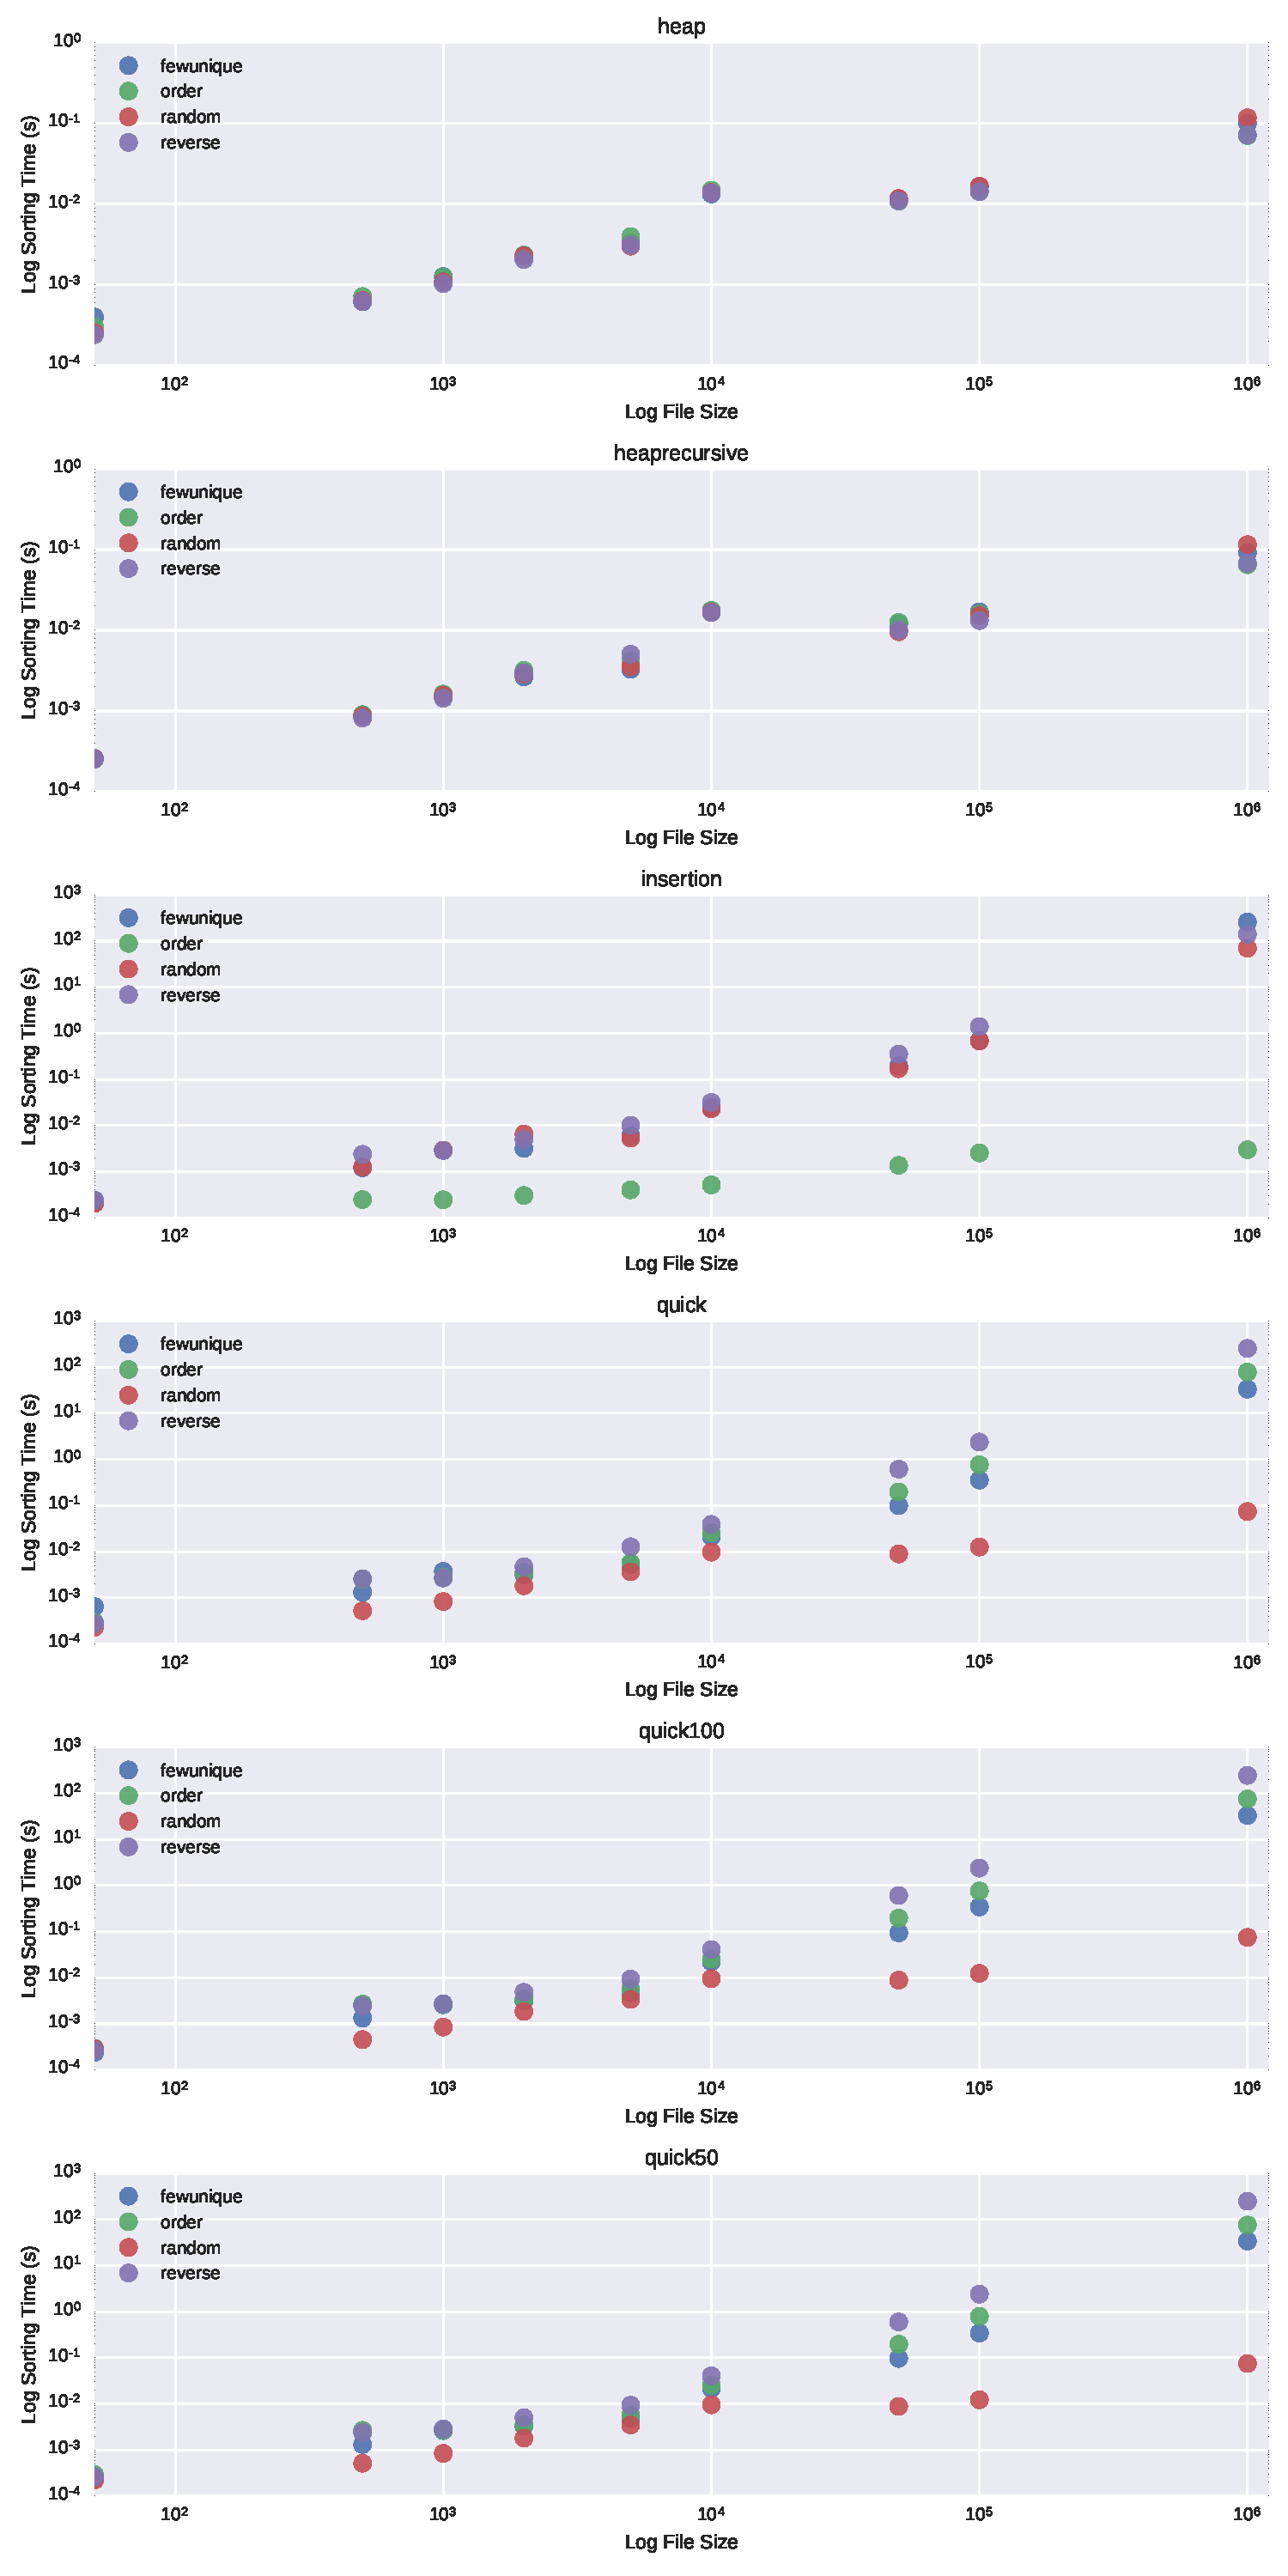
\includegraphics[width=.8\textwidth]{sorting_efficiency.pdf}
    \caption{Time complexity of the various sorting methods.  Note the variation in growth-rate at small sizes.}
    \label{fig:mesh1}
\end{figure}


%%%%%%%%%%%%%%%%%%%%%%%%%%%%%%%%%%%%%%%%%%%%%%%%%%%%%%%%%%

\section{What I learned}
The key take away from this lab is that sorting is not a "one size fits all" sort of problem.  From the timing alone, we can see that heap sort is a very good all-purpose sort.  Knowing nothing else, this would be a good sorting algorithm to employ.  However, if you know a little bit more about your input data, there are clear cases when an insertion sort would be a much better solution.  

From experiencing the development of the algorithms first-hand, developer time and possibility of bugs is also a huge factor.  Though insertion sort is often much slower than the other sorting methods, the incredible simplicity of the coding makes it much easier and quicker to implement a robust version.

%%%%%%%%%%%%%%%%%%%%%%%%%%%%%%%%%%%%%%%%%%%%%%%%%%%%%%%%%%

\section{Next time}
The biggest change to make to the next iteration of the code would be to allow sorting of more than simply integers.  Through dynamic typing
and generic comparisons, floats and strings could also be sorted and compared.  Though the work done was sufficient for the requirements of the lab, expanding this functionality would allow the code to be of greater use in the future.  

For a more expansive understanding of the costs of various sort methods, I would also like to implement additional sorting methods.  In particular, shell sort and merge sort would be two algorithms that would be good to know and enlightening to benchmark.


%%%%%%%%%%%%%%%%%%%%%%%%%%%%%%%%%%%%%%%%%%%%%%%%%%%%%%%%%%

\section{Timing Tables}
\begin{table}[h]
\caption {Ordered input data} 
\begin{tabular}{ccccccc}
size & heap & heaprecursive & insertion & quick & quick100 & quick50 \\ \hline
50 & 0.000302016 & 0.000258547 & 0.000239884 & 0.000294073 & 0.000295322 & 0.000292575 \\
500 & 0.000715298 & 0.000898571 & 0.0002481 & 0.002502428 & 0.002687569 & 0.002662073 \\
1000 & 0.001244428 & 0.001622032 & 0.000245037 & 0.002776963 & 0.002723678 & 0.002708003 \\
2000 & 0.002343468 & 0.003178912 & 0.000303522 & 0.003537735 & 0.003472342 & 0.003481398 \\
5000 & 0.003955591 & 0.004135522 & 0.000402162 & 0.005698625 & 0.00574016 & 0.00565567 \\
10000 & 0.014900791 & 0.017625875 & 0.000514676 & 0.025520635 & 0.025584726 & 0.025555939 \\
50000 & 0.010893812 & 0.012519946 & 0.001370123 & 0.196929157 & 0.196858958 & 0.197056017 \\
100000 & 0.014638626 & 0.015959849 & 0.002544921 & 0.768050875 & 0.765026838 & 0.787079903 \\
1000000 & 0.070613868 & 0.064917549 & 0.002985354 & 78.518782464 & 75.693605229 & 75.777595147 \\
\end{tabular}
\caption{Sorting time for the various methods on already sorted data.}
\end{table}


\begin{table}[h]
\caption {Reversed input data} 
\begin{tabular}{ccccccc}
size & heap & heaprecursive & insertion & quick & quick100 & quick50 \\
50 & 0.000240829 & 0.000252758 & 0.000240081 & 0.000276044 & 0.000265035 & 0.00026379 \\
500 & 0.000626288 & 0.000815482 & 0.002369405 & 0.00257659 & 0.002473359 & 0.002387058 \\
1000 & 0.00103394 & 0.001435553 & 0.002877741 & 0.002677203 & 0.002730043 & 0.002869858 \\
2000 & 0.002056936 & 0.002975382 & 0.004964522 & 0.004697828 & 0.004840655 & 0.005038788 \\
5000 & 0.003104991 & 0.005041868 & 0.010139983 & 0.012750024 & 0.009388691 & 0.009376173 \\
10000 & 0.013779397 & 0.016488256 & 0.031623458 & 0.038977392 & 0.040768036 & 0.040671503 \\
50000 & 0.010982646 & 0.010025143 & 0.352484684 & 0.614121943 & 0.606426719 & 0.59890119 \\
100000 & 0.014262541 & 0.013184438 & 1.407044154 & 2.38065916 & 2.386604456 & 2.395959443 \\
1000000 & 0.071852431 & 0.067870214 & 140.858910227 & 255.250420656 & 244.969556828 & 248.237793146 \\
\end{tabular}
\caption{Sorting time for the various methods on reverse sorted data.}
\end{table}

\begin{table}[h]
\caption {Random input data} 
\begin{tabular}{ccccccc}
size & heap & heaprecursive & insertion & quick & quick100 & quick50 \\
50 & 0.00025382 & 0.000256079 & 0.000204695 & 0.000229099 & 0.000289335 & 0.000222816 \\
500 & 0.000641477 & 0.000861359 & 0.001262513 & 0.000523076 & 0.000455218 & 0.000514021 \\
1000 & 0.001087033 & 0.001559881 & 0.002927089 & 0.000829874 & 0.000852996 & 0.000843831 \\
2000 & 0.00228379 & 0.002893117 & 0.006512311 & 0.00182818 & 0.001856103 & 0.001804946 \\
5000 & 0.003016992 & 0.003538806 & 0.005306821 & 0.003661825 & 0.00341101 & 0.003473115 \\
10000 & 0.01390287 & 0.016773763 & 0.023102573 & 0.009766037 & 0.009586525 & 0.009552995 \\
50000 & 0.011742627 & 0.009586244 & 0.170864514 & 0.008918867 & 0.008888181 & 0.008818398 \\
100000 & 0.016668384 & 0.015165901 & 0.682780545 & 0.012587182 & 0.012452452 & 0.012267705 \\
1000000 & 0.117493548 & 0.115109439 & 70.007879439 & 0.074078908 & 0.075245845 & 0.075035085 \\
\end{tabular}
\caption{Sorting time for the various methods on random sorted data.}
\end{table}

\begin{table}[h]
\caption {Few unique input data} 
\begin{tabular}{ccccccc}
size & heap & heaprecursive & insertion & quick & quick100 & quick50 \\
50 & 0.0003978 & 0.000252842 & 0.000207553 & 0.000643817 & 0.000239713 & 0.000242833 \\
500 & 0.000615428 & 0.000882167 & 0.001215953 & 0.001310385 & 0.001325422 & 0.001313499 \\
1000 & 0.001267839 & 0.001524172 & 0.00287119 & 0.003733475 & 0.002603169 & 0.002635834 \\
2000 & 0.002315942 & 0.002647341 & 0.003195627 & 0.003146445 & 0.003144586 & 0.00328196 \\
5000 & 0.003310394 & 0.003272234 & 0.005934386 & 0.005229633 & 0.004822836 & 0.00484362 \\
10000 & 0.013390662 & 0.01710462 & 0.024208983 & 0.021325309 & 0.022190923 & 0.021652428 \\
50000 & 0.011519663 & 0.012020441 & 0.197074721 & 0.099174622 & 0.094072075 & 0.096792049 \\
100000 & 0.016533855 & 0.016950739 & 0.69644773 & 0.356080076 & 0.343005856 & 0.34397153 \\
1000000 & 0.100491692 & 0.091801463 & 259.352003426 & 33.30067469 & 33.079817714 & 33.792895479 \\
\end{tabular}
\caption{Sorting time for the various methods on data with duplicates.}
\end{table}

\end{document}
